\documentclass{ledger}



\newcommand{\thefirstpagenum}[0]{X}
\newcommand{\thelastpagenum}[0]{X}
\newcommand{\theyear}[0]{20XX}
\newcommand{\thevol}[0]{X}
\newcommand{\thedoi}[0]{DOI 10.5195/LEDGER.\theyear.XXX}
\newcommand{\ledgerpages}[0]{\thefirstpagenum-\thelastpagenum}
\newcommand{\nxn}[1]{$#1 \times #1$}
\usepackage{float}
\usepackage{graphicx}
\usepackage{adjustbox}
\usepackage{pdflscape}
\usepackage{svg}
\usepackage{amsmath}
\usepackage{listings}
\usepackage{xcolor}
\usepackage{tocloft}
\usepackage{hyperref}
\usepackage{attachfile}



\definecolor{codegreen}{rgb}{0,0.6,0}
\definecolor{codegray}{rgb}{0.5,0.5,0.5}
\definecolor{codepurple}{rgb}{0.58,0,0.82}
\definecolor{backcolour}{rgb}{0.95,0.95,0.92}


\lstdefinestyle{mystyle}{
    backgroundcolor=\color{backcolour},   
    commentstyle=\color{codegreen},
    keywordstyle=\color{black},
    numberstyle=\tiny\color{codegray},
    stringstyle=\color{codepurple},
    basicstyle=\ttfamily\footnotesize,
    breakatwhitespace=false,         
    breaklines=true,                 
    captionpos=b,                    
    keepspaces=true,                 
    numbers=left,                    
    numbersep=5pt,                  
    showspaces=false,                
    showstringspaces=false,
    showtabs=false,                  
    tabsize=2
}

\lstset{style=mystyle}
%\usepackage[pdftex,pdfpagelabels,bookmarks,hyperindex,hyperfi%gures]{hyperref}.
%AUTHOR: please set these to generate correct PDF metadata
\hypersetup{pdfauthor={Prusak, Patryk;}, pdftitle={AIF-Project}}

%EDITOR: set the correct pageination during layout
% \setcounter{page}{\thefirstpagenum}


%AUTHOR: this can be used to highlight changed text, surround with \edit{} and
%uncomment either to determine color
%\newcommand{\edit}[1]{{\color{red} #1}}
\newcommand{\edit}[1]{#1}
	
\overfullrule=10pt

\title{Project of emotion classifier based on text and image data}
\author{\normalsize Weronika Piotrowska, Marcin Wojnarowski, Mikołaj Stańczyk, Patryk Prusak}

\pagestyle{pagemain}
% 


%The Author should select the appropriate pretitle below:
\pretitle{
  \centering \selectfont Artificial Intelligence Fundamentals \par
  %\centering \selectfont REVIEW ARTICLE \par
  %\centering \selectfont RESEARCH ARTICLE \par 
  \fontsize{24pt}{28pt}\selectfont} % Title is centered and at 24pt


\begin{document}

\maketitle

\thispagestyle{pagefirst}

\begin{abstract}
	Implementation of emotion detection/classification based on text and images separately using statistical and machine learning models. Together with a discussion and comparison to existing solutions, results are presented.

	\begin{keywords}
		\item Emotion Detection
		\item Machine Learning
		\item Artificial Intelligence
	\end{keywords}
\end{abstract}
\begin{figure}[hb]
	\centering

	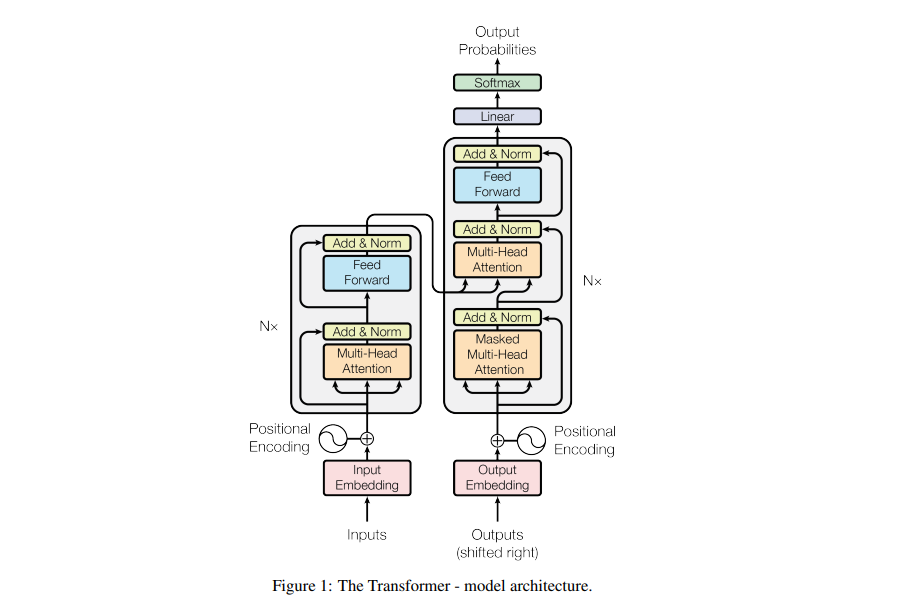
\includegraphics[width=\textwidth]{assets/transformer.png}
\end{figure}

\clearpage
\tableofcontents

\newpage

\section{Introduction}

There are many approaches to automatic emotion recognition. Even though a significant progress has been made in the recent years, human emotions still remain complex, ambiguous and thus incomprehensible for the machines. The goal of creating a neural network capable of recognizing human emotions based on speech, text or facial expression is still a challenging task. Our approach to this problem will be not only to use photographic images, but also short text, such as Tweets.

\section{Problem Analysis}

Text based emotion detection remains a complicated task due to its strongly reliance on Natural Language Processing (NLP) which is known to be hard to generalize. Human speech (or in this case writing) might seem structured and therefore easy to study, but that unfortunately is far from the truth. We humans rely on intuition which is notoriously hard to reason about for machines trying to abstract these notions. NLP has many approaches to it, but two stand out:

\begin{enumerate}
	\item Probabilistic statistical models -- these base their reasoning purely only the previously analyzed data and provide prediction based on the most probable outcome. These generalize poorly, but can provide very solid results for a contained goal.

	\item Deep learning models -- with the recent boom in deep learning, it of course has influenced NLP as well. Popular models such as BERT or GPT-3 belong to the largest deep learning models ever which shows the great complexity of the task at hand. These generalize much better, but are much more computationally expensive\cite{https://doi.org/10.48550/arxiv.2005.00547}.
\end{enumerate}
\noindent
The problem of computer-assisted emotion recognition based on images has been moderately studied, resulting in many attempts, some of them with decent results. This fact presents us with many approaches we could use and hopefully improve. The basic process of finding an emotion from a picture goes as follows:

\begin{figure}[H]
	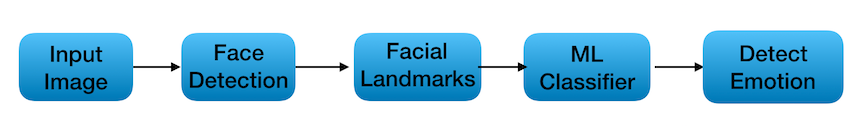
\includegraphics[width=15cm]{assets/emotion_recognition_process.png}
	\caption{Example process of image emotion detection}
	\centering
\end{figure}

Despite it's popularity, this area has a big potential for new inventions and applications, which we are happy to explore in this project.

\section{Applications}

\subsection{Image Emotion Recognition}
It is commonly thought that each of us is rather skilled at recognizing each others emotions, however, that is often not the case. Even trained individuals, like therapists, find it difficult to decipher patient's mood and their conclusions are often way off the mark. And so emotion recognition software could be a great asset to professionals willing to better understand their patients and improve the effectiveness of therapy. Such product has the potential to gain on popularity in the coming years because the area of mental health undergoes a small revolution, in a sense that it is being digitalized.

\subsection{Text Emotion Recognition}

Text emotion detection has many applications including automatic moderation. Large companies might want to filter out comments which talk about the company using negative sentiments, or filter in those with positive sentiments. Other than filtering, it can give a very quick feedback regarding a matter. For example \textit{The Body Shop} uses a sentiment analysis tool \textit{Brandwatch} to gather the general reception of a campaign\footnote{\url{https://www.brandwatch.com/case-studies/the-body-shop/view/?utm_source=google&utm_medium=cpc&utm_campaign=sentiment_analysis}}.

\hfill

If both image recognition and text recognition will produce satisfying results, we can combine the two. For example, one can base the user's sentiment not only on the Tweet they wrote, but also on the picture attached. Furthermore, it can be broaden to using videos as the input data, compiling both images and text. However, this solution would require additional algorithms and computing power, in order to extract image frames from the video and text from speech data.

\section{Existing Solutions}

\subsection{GoEmotions}
Emotion detection from text has been tackled multiple times before. One notable project is the GoEmotions by Google Research. It created a multi-classification model based on the BERT model for reddit comments. As the authors have described, getting clean, representative data was a challenge\cite{https://doi.org/10.48550/arxiv.2005.00547}. Reddit has a known demographic bias leaning towards young male users, which skews the data towards a toxic, offensive language. This is aligned with problems which we observed, that is, a high quality representative NLP dataset is hard to obtain. GoEmotions focused on 28 different emotions (Fig. \ref{fig:goemotions-classes}) and assigned to a given text a probable combination.

\begin{figure}[H]
	\centering
	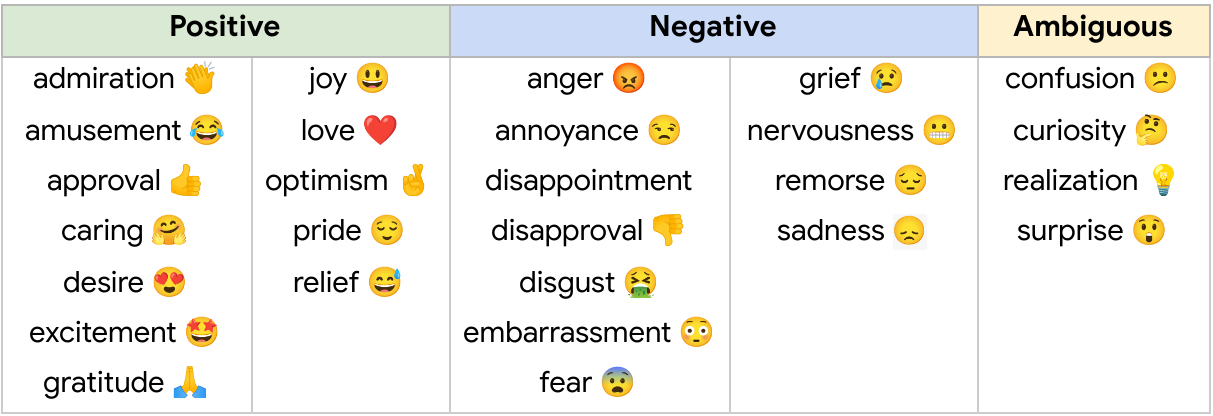
\includegraphics[width=1\textwidth]{assets/goemotions_classes.png}
	\caption{GoEmotions 28 emotion classes}
	\label{fig:goemotions-classes}
\end{figure}

\subsection{Twitter-roBERTa-base for Emotion Recognition}
This solution, based on roBERTa model\footnote[3]{\url{https://doi.org/10.48550/arxiv.1907.11692}} using TweetEval benchmark\footnote[4]{\url{https://doi.org/10.48550/arxiv.2010.12421}} distinguishes between four emotions: joy, optimism, anger and sadness. As the output, it gives the user probability with which the model predicted certain emotions.\footnote[2]{\url{https://huggingface.co/cardiffnlp/twitter-roberta-base-emotion}}

\begin{figure}[H]
	\centering
	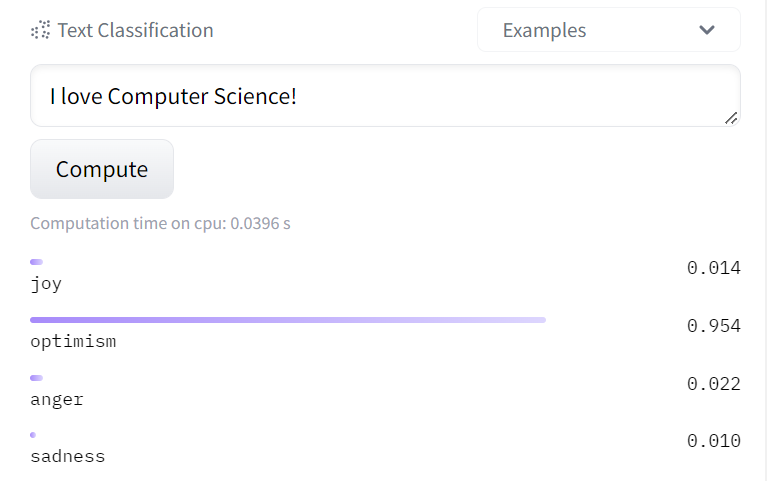
\includegraphics[width=1\textwidth]{assets/roberta.png}
	\caption{Sample output from the model}
	\label{fig:goemotions-classes}
\end{figure}
\subsection{Multi-class Emotion Classification for Short Texts}
The approach presented in this solution uses LSTM and CNN models, classifying int five classes: neutral, happy, sad, anger, hate. The authors achieved 62.29\% accuracy.\footnote[2]{\url{https://tlkh.github.io/text-emotion-classification/}}

\subsection{Meta-learning}
The authors have used CMU MULTI-PIE dataset which contains images with different head-poses, occlusions and illumination levels. The used method is called ERMOPI(Emotion Recognition using Meta-learning across Occlusion, Pose and Illumination) that detects emotion from faces using meta-learning approach and works well with partial occlusions, different head poses and illumination levels. The key benefit of this approach is the decreased need for training samples compared to existing solutions to emotion recognition and at the same time, very reliable results. This approach achieved 90\% accuracy for CMU Multi-PIE images and 68\% for AffectNet images.\footnote[3]{\url{https://www.sciencedirect.com/science/article/pii/S1319157821001452}}

\subsection{The Face Emotion Recognizer}
This is an open-source Python library built and maintained by Justin Shenk. It uses a convolutional neural network with weights contained in the HDF5 file. This project offers the possibility to use MTCNN (multi cascade convolutional network) to detect faces or the default OpenCV Haarcascade classifier. It detects emotions in six categories: fear, neutral, happy, sad, anger and disgust.\footnote[1]{\url{https://towardsdatascience.com/the-ultimate-guide-to-emotion-recognition-from-facial-expressions-using-python-64e58d4324ff}}

\subsection{Deep-Emotion}
This paper presents an deep learning approach based on attentional convolutional networks in order to tackle more difficult images such as datasets with partial faces. The model is able to focus on crucial parts of the face to detect emotions. It achieves significant improvement over previous models in datasets such as FER-2013 or FERG. This method also shows that different emotions are sensitive to different parts of human face.\footnote[2]{\url{https://mdpi-res.com/d_attachment/sensors/sensors-21-03046/article_deploy/sensors-21-03046.pdf?version=1619511102}}

\section{Chosen Solution}

\subsection{Datasets}

For the emotion recognition based on images, we have chosen the FER-2013 dataset\footnote{\url{https://www.kaggle.com/msambare/fer2013}} (Fig. \ref{fig:fer2013}). Facial Expression Recognition 2013 contains 35,887 facial gray-scale images (pre-split into 80/20 train/test set) of different expressions with size restricted to 48×48. Main labels assigned to pictures can be divided into 7 categories:

\begin{enumerate}
	\item Angry
	\item Disgust
	\item Fear
	\item Happy
	\item Sad
	\item Surprise
	\item Neutral
\end{enumerate}

\begin{figure}[H]
	\centering
	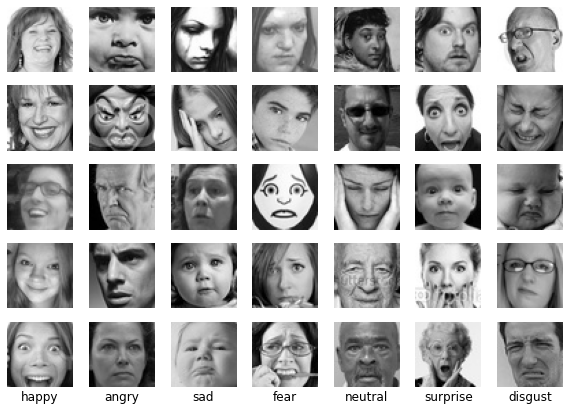
\includegraphics[width=0.7\textwidth]{assets/fer2013.png}
	\caption{A sample of the FER2013 dataset grouped by their respective emotions}
	\label{fig:fer2013}
\end{figure}

We can quickly notice a few things. Firstly, the faces seem nicely centered though even if they weren't CNNs inherently are translate-invariant so it would not be a problem. Secondly, the training and testing set does not seem to differ substantially.

On the other hand, many issues can be identified:

\begin{enumerate}
	\item  Many of the pictures are stock pictures where the emotion is grossly exaggerated. This may cause the model to fail to learn the subtleties of how an emotion is expressed.
	\item Different scales/rotations. Kernels in a CNN are not scale/rotation-invariant and will fail to generalize for different sizes/rotations of studied objects (lips, eyebrows, etc). Layers such as maxpooling are said to be helping here \footnote{Deep Learning. Ian Goodfellow and Yoshua Bengio and Aaron Courville -- \url{https://www.deeplearningbook.org}}
	\item Different lightning conditions.
	\item Mixture of real pictures with computer drawn.
	\item All previous arguments are technical limitations which can be overcome. However, one last important problem which can be noticed is that some of these emotion labels are very debatable. Me (as a fellow human) would fail to classify some of those to the associated label.
\end{enumerate}

With all of that in mind, and our expectations being managed we proceeded to prepare our model.

Each label has about 4,000 samples each besides \textit{disgust} that has about 600 images (Fig. \ref{fig:images-classes}).

\begin{figure}[H]
	\centering
	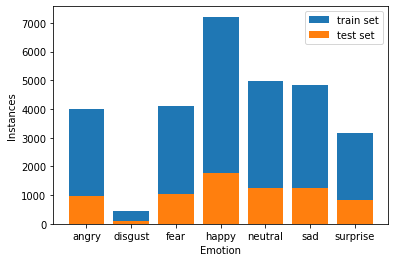
\includegraphics[width=0.7\textwidth]{assets/image_dataset.png}
	\caption{Distribution of classes in the FER-2013 dataset.}
	\label{fig:images-classes}
\end{figure}


Similarly, we have chosen a text dataset to portray similar emotions. We are using \emph{Predict emotion from textual data : Multi-class text classification} published on Kaggle\footnote{\url{https://www.kaggle.com/datasets/pashupatigupta/emotion-detection-from-text}}.
The dataset contains 40,000 short text messages scrapped from Twitter. Each of them were labeled by human employees, distinguishing the following emotions as seen on Fig. \ref{fig:textds-classes}.

\begin{figure}[H]
	\centering
	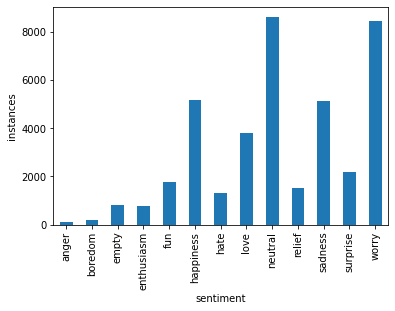
\includegraphics[width=0.7\textwidth]{assets/text_dataset_classes.png}
	\caption{Amount of instances per class}
	\label{fig:textds-classes}
\end{figure}

One can immediately notice that the proposed dataset is very imbalanced - this, we have decided to merge similar classes (e.g. happiness and fun) and drop classes that are not useful. The final processed dataset we will be working on looks as follows:
\begin{enumerate}
	\item Happiness
	\item Love
	\item Neutral
	\item Sadness
	\item Worry

\end{enumerate}

We have chosen

\hfill

\subsection{Libraries}
To recognise emotions from images following libraries will be used:
\begin{itemize}
	\item{} \href{https://numpy.org}{NumPy} - for vectorized operations on arrays
	\item{} \href{https://keras.io}{keras} - software library providing Python interface for artificial neural networks
	\item{} \href{https://www.tensorflow.org/}{tensorflow} - Google's machine learning framework. Both the python and JS versions will be used

\end{itemize}

To recognise emotions from text following libraries will be used:
\begin{itemize}
	\item{} \href{https://numpy.org}{NumPy} - for low level vectorized arrays
	\item{} \href{https://pandas.pydata.org}{pandas} - used for data frames manipulation and analysis
	\item{} \href{https://www.nltk.org/}{nltk} - library which implements models for text analysis

\end{itemize}

\subsection{Models}

For image emotion detection we converged onto a deep but classical Convolutional Neural Network with strong regularization. As seen on Fig. \ref{fig:images-model} the final model consists of interleaved convolutional layers with max pooling layers. Every block contains a batch normalizer to keep the computations numerically stable as well as a 25\% dropout layer for regularization. Occasionally an L2 regularizer is applied to some layers to further ensure regularization. Finally, all layers use the rectified linear unit as an activation function to introduce non-linearity, this particular choice is from the simple fact that it seems to be the industry standard. After spatial feature extraction with convolutional layers is done, the output is flattened and passed to a 3-layered dense fully-connected network which outputs the final class prediction as a softmax probability distribution. The goal function to minimize will be the categorical cross entropy function, and the optimizer used is the stateful Adam optimizer.

As an additional regularizer, training images are randomly rotated, scaled, and flipped horizontally to introduce noise.


\hfill

For the text classification, we will use nltk's pre-trained Naive Bayes Classifier, which is based on naive Bayes algorithm. The algorithm makes 'naive' assumption that all labels are independent, so the following equation holds:

\[P(label|features) = \frac{P(label)\cdot P(f_1|label) \cdot \ldots \cdot P(f_n|label)}{P(features)}\]

The algorithm computes probability for each label and returns the label that fits the given test the best.

\begin{figure}[H]
	\centering
	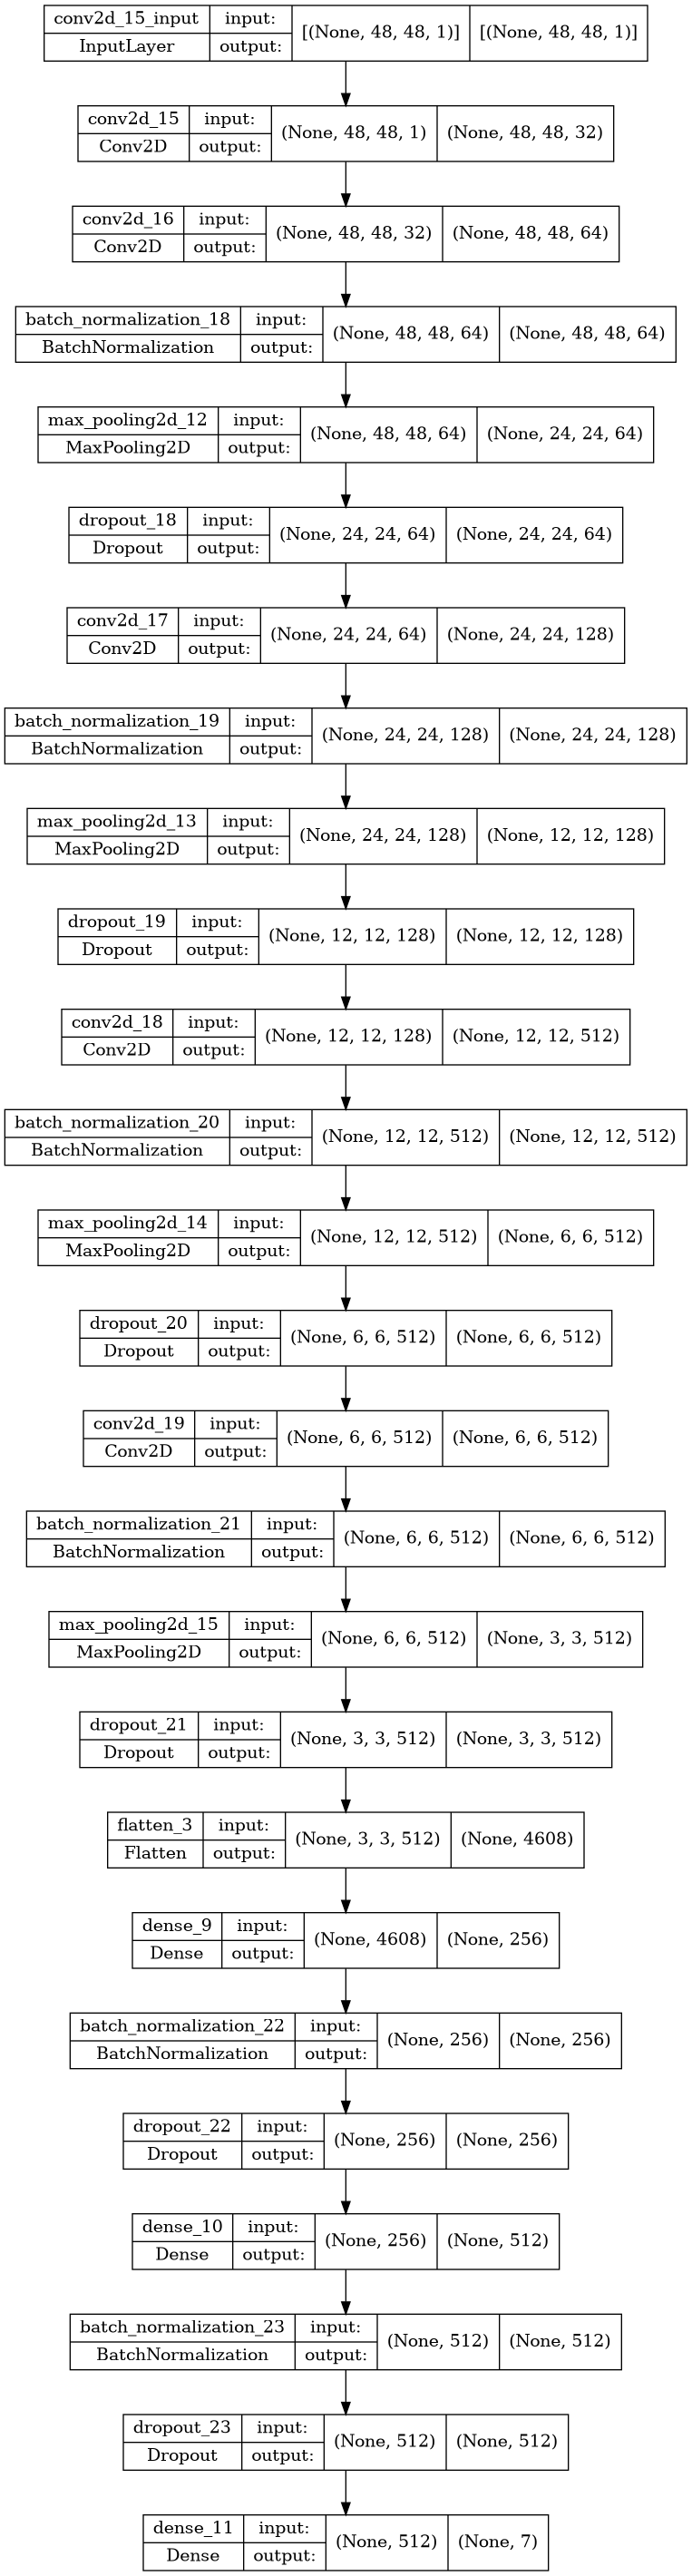
\includegraphics[width=0.4\textwidth]{assets/images_model.png}
	\caption{Visual representation of the final image emotion detection model}
	\label{fig:images-model}
\end{figure}



\section{Results}

The 4.5 million parameter image model was trained for about 3 hours in \href{https://research.google.com/colaboratory}{Google Colab} using their free GPU resources. A total of 200 epochs were completed with constant validation set checks. Final results are presented bellow

\begin{itemize}
	\item Train set -- loss: 0.6216, accuracy: 80.03\%
	\item Test set -- loss: 1.0202, accuracy: 66.98\%
\end{itemize}

Notice, that a result of 67\% for emotion recognition is not a bad result: after all, emotions are ambiguous and often hard to describe with just a single term. Perhaps multi-classification would prove to be better for such a task. Additionally, emotions are far from being linearly different. That is, sadness and neutrality do not differ greatly when expressed facially. On the other hand, happiness and angriness are much more distinct. Classes have different distances between each other.



\begin{figure}[H]
	\centering
	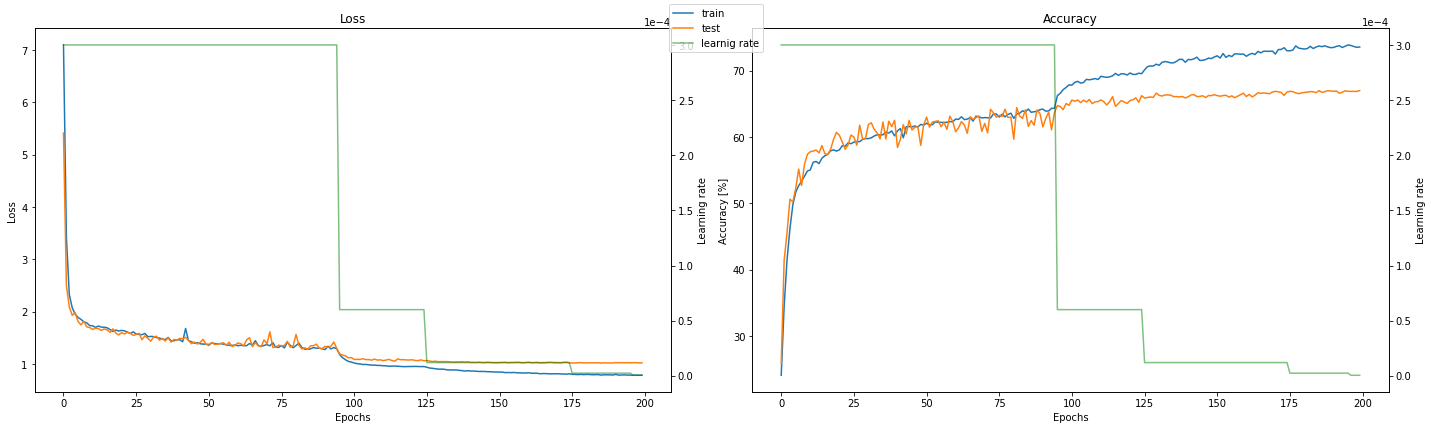
\includegraphics[width=1\textwidth]{assets/image_training_results.png}
	\caption{Training history for the train and validation set. Two measures: loss (left), accuracy (right).}
	\label{fig:image-training-results}
\end{figure}

In Fig. \ref{fig:image-training-results} we can immediately notice a few interesting things: the model learns to classify images effectively within just a few initial epochs. Afterwards the improvement slows down dramatically. After the first learning rate decrease we can notice a sudden improvement in both sets. While initially the loss does not diverge in a significant matter between the sets, at around epoch 125 (when the second learning rate drop is applied) we can notice that the test set (here used as a validation set) no longer reports improvements and the model is clearly starting to overfit the dataset.


The learning rate reductions clearly show the model reaching a more stable performance. Ideally, training should be stopped either right after the first LR drop, or right before the second one.

\begin{figure}[H]
	\centering
	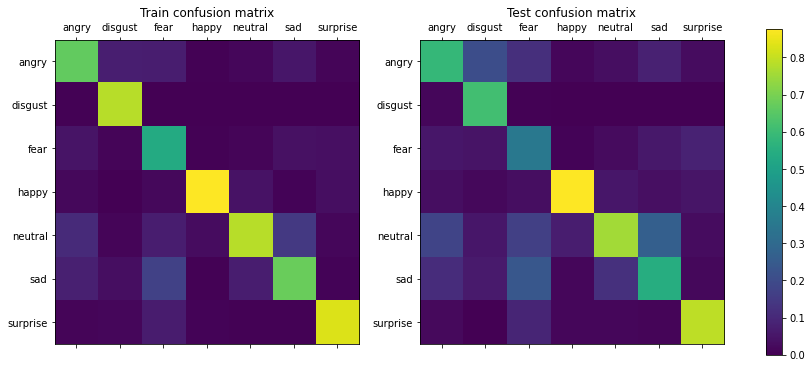
\includegraphics[width=1\textwidth]{assets/image_conf_matrix.png}
	\caption{Confusion matrix for the final image model. Separately for the training set (left) and testing set (right).}
	\label{fig:image-conf-mat}
\end{figure}

Finally, the confusion matrix is shown (Fig. \ref{fig:image-conf-mat}). X-axis depicts the label and the y-axis plots the distribution of the model's predictions. As expected the brightest parts are on the diagonal (true positives). Train's and test's confusion matrices exhibit a similar pattern, which enforces the belief that the model managed to not overfit the train set. The brightest class seems to be 'happy', which was predicted correctly 87\% of the time in the test set and 94\% in the train set. The small amount of examples of disgust is visible here: when y=disgust, x is only bright for disgust. Occasional brighter parts outside of the diagonal can be observed, these can be probably attributed to ambiguous pictures; the biggest confusion seems to be classifying fear as sadness, and classifying sadness as neutrality.

\hfill

For the text emotion detection, the results were not satisfactory. The model obtained 39\% accuracy, which was very low. The model found the most informative words, that is, words that strongly indicate the class, to be as follows:

\begin{figure}[H]
	\centering
	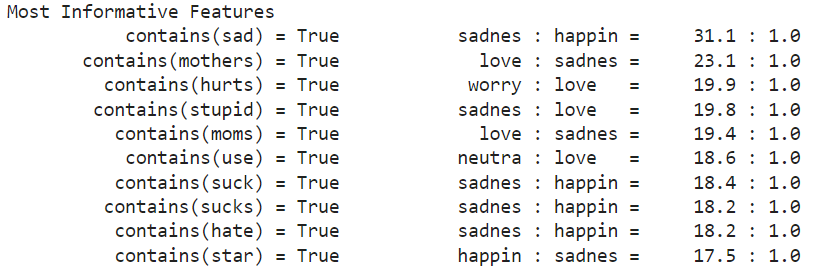
\includegraphics[width=1\textwidth]{assets/text_inf_features.png}
	\caption{The most informative features (words) given by the model.}
	\label{fig:image-training-results}
\end{figure}


\subsection{Demo}

Using the trained model a demo app was prepared which recognizes emotions in real time (60 times per second) from a camera feed. The app was written in TypeScript using the JS interface of Tensorflow called Tensorflow.js. There, the exported keras model was imported and warmed up in the WebGL environment. The webcam is started and each frame is streamed through the recognition pipeline. First, using the blazeface model\cite{https://doi.org/10.48550/arxiv.1907.05047} a face is detected (or not) and the bounding box is returned. If a face was found, the image is cropped to the face and normalized to the expected input of our model (apply grayscale filter, resize, and reshape). Once done, the face image is fed to our model and a prediction is made and finally displayed (Fig. \ref{fig:demo}). In this case the label was determined based off the argmax of the final softmax layer, there was no threshold.

\begin{figure}[H]
	\centering
	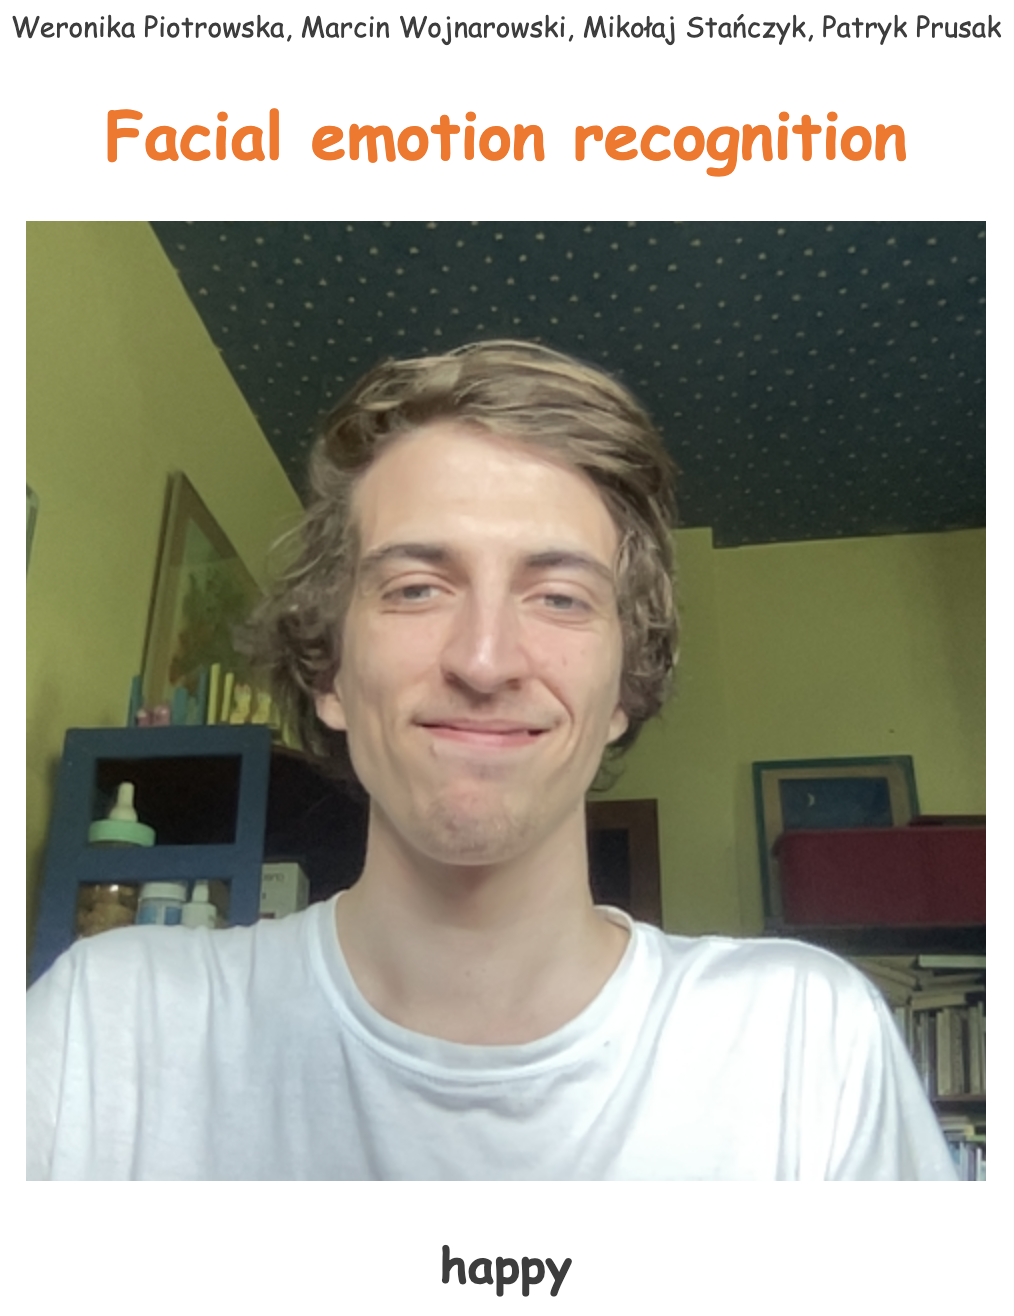
\includegraphics[width=0.7\textwidth]{assets/demo.png}
	\caption{Demo app deployed to be available online}
	\label{fig:demo}
\end{figure}

Additionally, the app can run in debug mode where the normalized image is shown together with the full prediction distribution (Fig. \ref{fig:demo-debug}).

\begin{figure}[H]
	\centering
	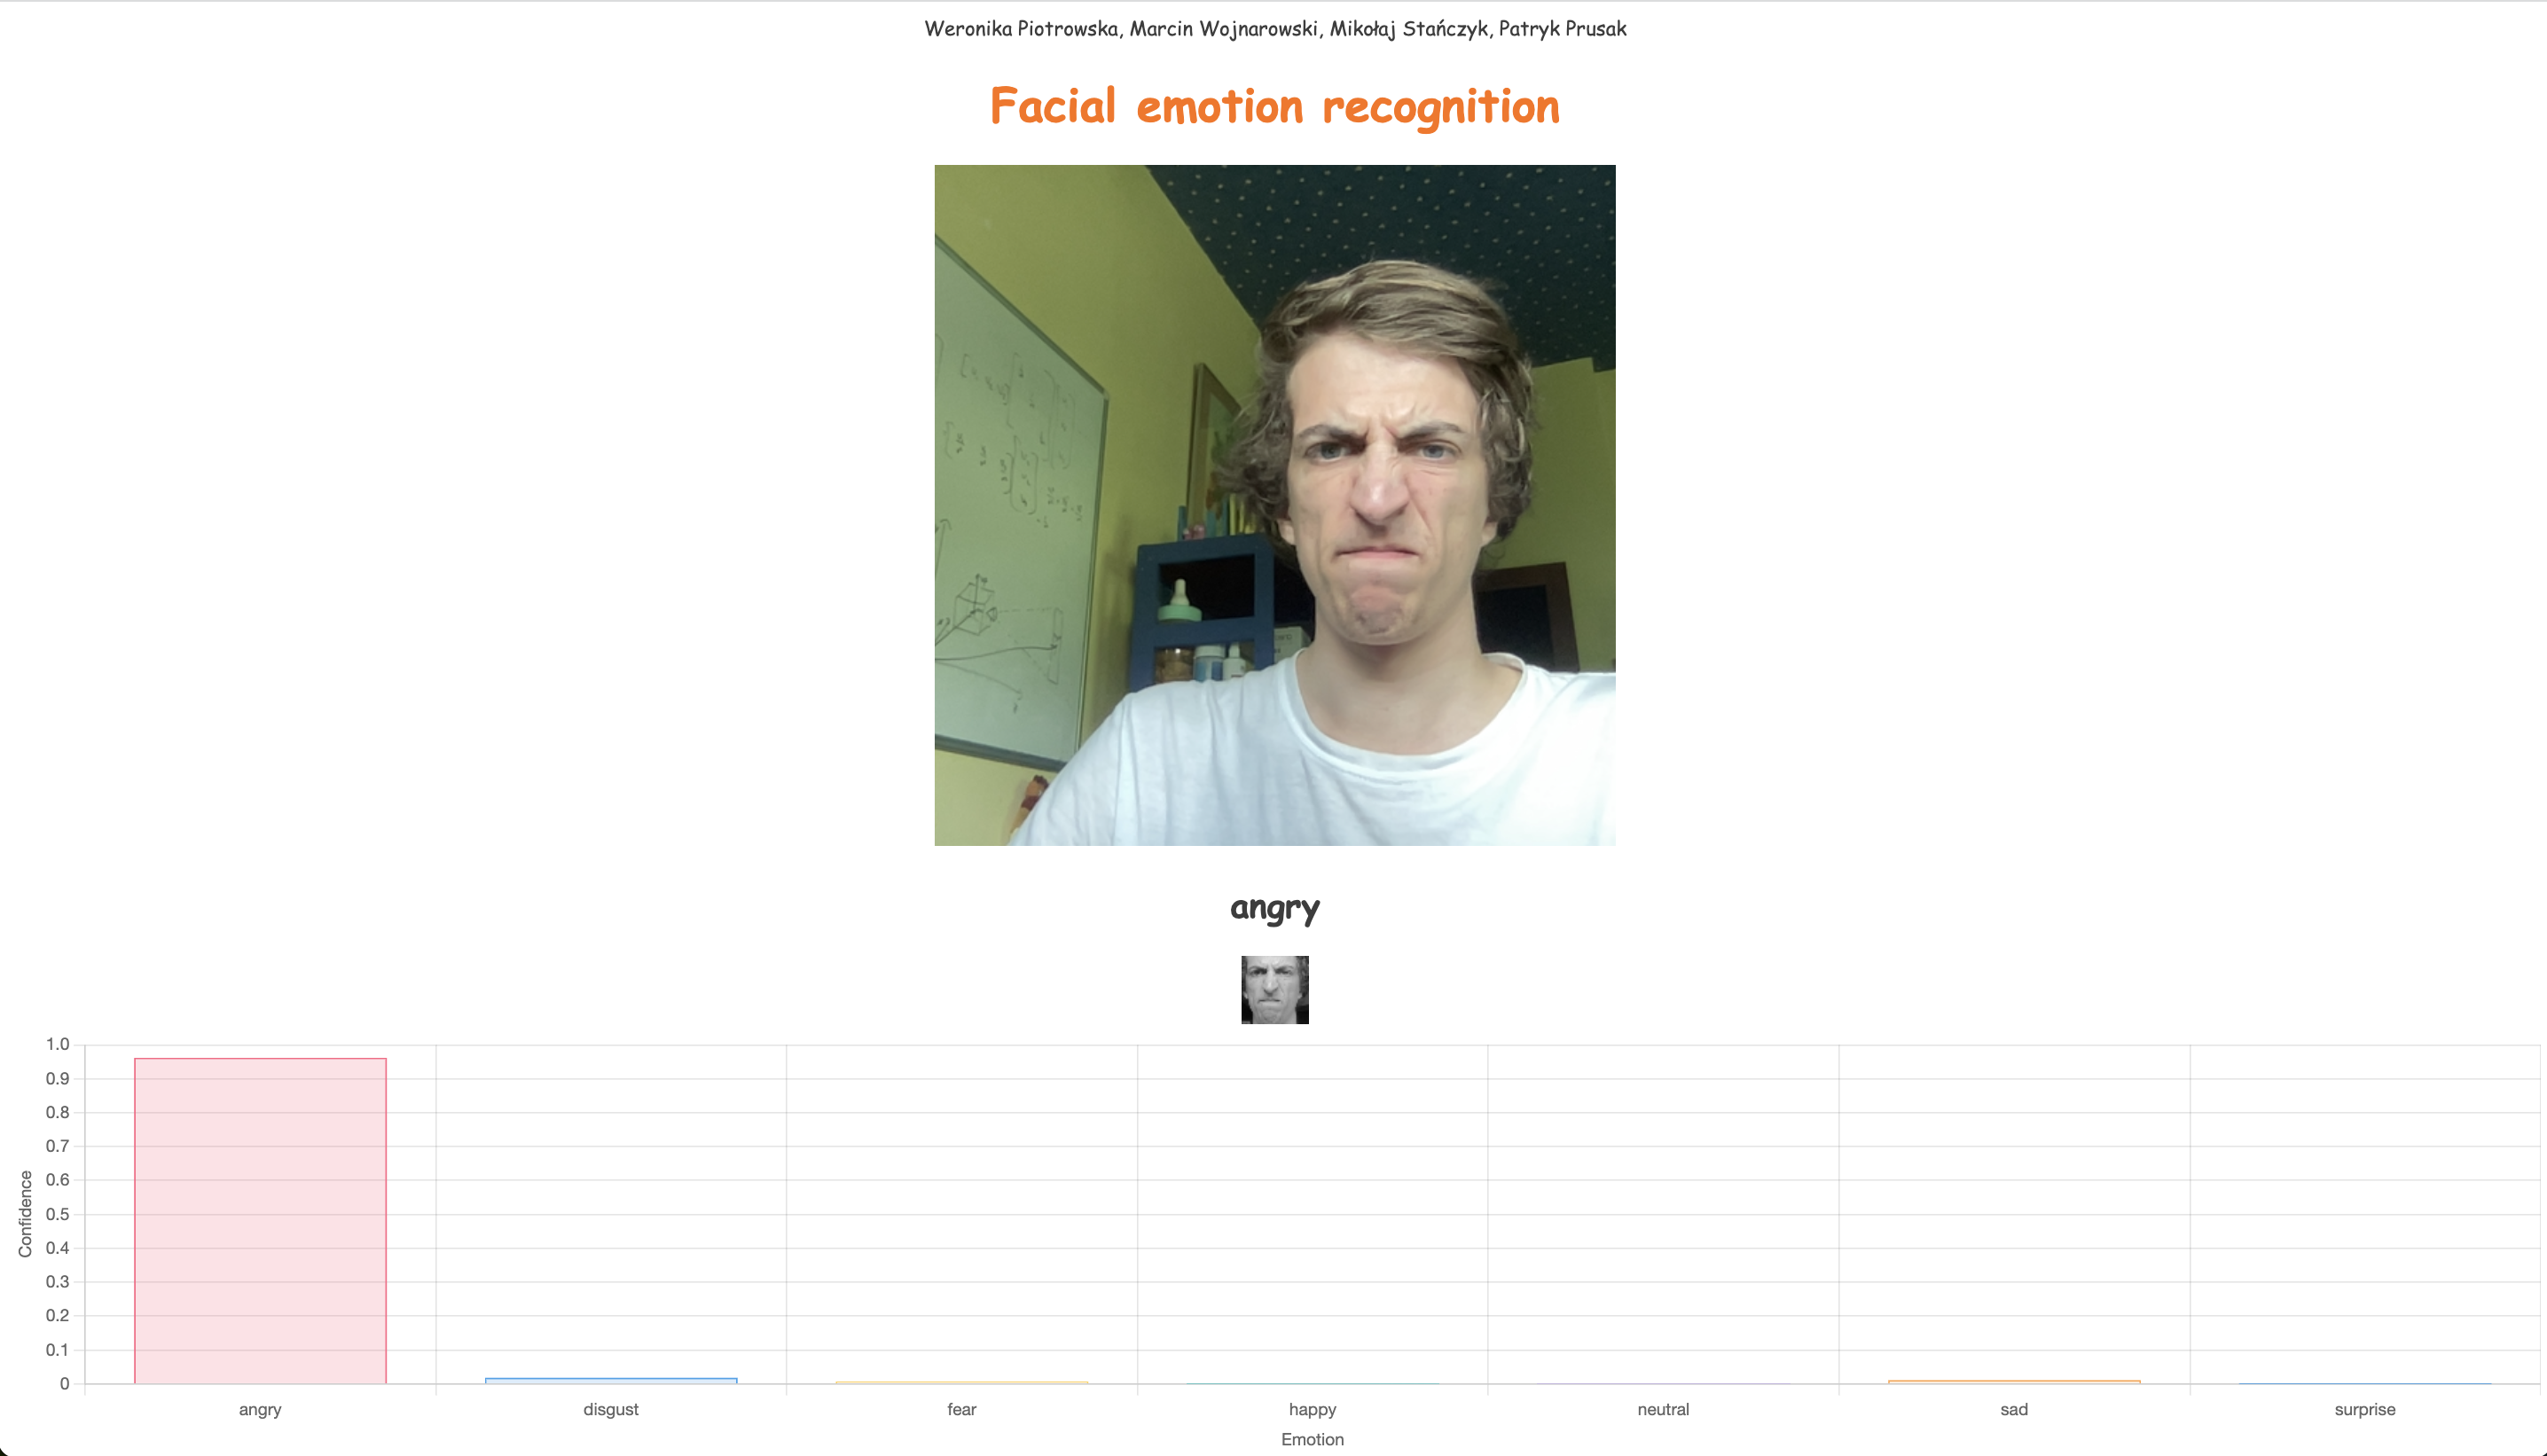
\includegraphics[width=1\textwidth]{assets/demo-debug.png}
	\caption{Demo app showing the normalized input image and the output distribution}
	\label{fig:demo-debug}
\end{figure}

\section{Conclusion}

The results obtained from the image emotion recognition are very satisfactory. Despite the reported accuracy of only 67\%, in practice the model yielded very accurate predictions. In the prepared demo, the model fared well and was able to predict emotions very often. Drawbacks of our solution include a poor dataset (emotions are exaggerated) which causes it to fail to recognize subtle hints of emotions, and a not-so-sophisticated model (deep, but basic).

\hfill

However, the results obtained from text emotion recognition were not satisfactory. The model obtained 39\% accuracy on the test set. We suspect the failure was because of wrongly labeled dataset, since some samples were labeled by two labels. Also, while analyzed the data, we found that the labels were sometimes not accurate for the given sample.

Due to that, we decided to not include text emotion recognition model in our GUI.

\section{Attachments}

\begin{enumerate}
	\item {\textattachfile[color=0 0 1]{text_src.zip}{text\_src.zip} -- Source code of the text emotion detection notebook}
	\item {\textattachfile[color=0 0 1]{image_src.zip}{image\_src.zip} -- Source code of the image emotion detection notebook}
	\item {\textattachfile[color=0 0 1]{demo_src.zip}{demo\_src.zip} -- Source code of the demo for real-time webcam emotion detection}
	      \item{} \url{https://github.com/shilangyu/AIF-emotion-detection} -- repository with all the whole work
\end{enumerate}


\bibliographystyle{ledgerbib}
\bibliography{tempbib}

\end{document}
